\chapter{Scale-Covariant Refinement Dark Sector}
\label{ch:scale-covariant-dark-sector}

\begin{monographnote}[Production hypothesis]
The rapid-crossing formulas in this chapter describe a specified-background approximation. The covariant fiber analysis shows that the benchmark spectrum overdraws its available energy. Its normalized shape is therefore an input to downstream transport, not an established solution of the coupled production problem.
\end{monographnote}
\section{Scope and objective}

The preceding unified dark-sector model used an additive average-detail Hessian,
\begin{equation}
 m_h^2(\phi)=m_h^2+3\lambda\phi^2,
 \label{eq:scw-additive-mass}
\end{equation}
so that a light produced shell could both cluster and stabilize the average mode.  A hard abundance and coldness audit exposes a restricted but serious obstruction in that branch.  On an energy-matched rapid crossing, one dominant additive shell cannot simultaneously reproduce the present dark abundance, remain nonrelativistic, and lock the average mode.

This chapter first proves that obstruction under its stated hypotheses.  It then replaces the additive Hessian by one scale-covariant deformation of the whole refinement operator,
\begin{equation}
 \mathcal L_{\sigma,p}
 \longmapsto
 \left(1+\gamma\frac{\phi^2}{v^2}\right)\mathcal L_{\sigma,p}.
 \label{eq:scw-scale-covariant-rule}
\end{equation}
The replacement introduces one dimensionless coupling $\gamma$, not an independently chosen coupling at every level.  It has two linked effects:
\begin{enumerate}[leftmargin=2em]
\item heavier detail levels are created with proportionally broader nonadiabatic scales and become colder after redshift;
\item the same weighted detail energy, rather than the inverse-mass variance of one light shell, stabilizes the average mode.
\end{enumerate}

The resulting branch supplies an analytic mass envelope, an exact captured rest-energy fraction, a derived late-time equation of state, a dark-density locking law, and a one-parameter small-scale cutoff family.  The scale-covariant coupling itself is a model extension.  It is not claimed to follow uniquely from the primitive projector axioms.

\section{Additive one-shell obstruction}

Let
\begin{equation}
 \rho_V=\frac{\mu^4}{4\lambda},
 \qquad
 m=\alpha\mu,
 \qquad
 \beta=\frac{\nu}{\mu^2},
 \qquad
 r_D=\frac{\rho_{D0}}{\rho_V}.
 \label{eq:scw-additive-definitions}
\end{equation}
Assume one shell of degeneracy $g$ is populated at scale factor $a_\star$ by the energy-projected Gaussian
\begin{equation}
 f(q)
 =\eta
 \exp\left[
 -\frac{\pi m^2}{\nu}
 -\frac{\pi q^2}{a_\star^2\nu}
 \right],
 \qquad
 0<\eta\leq1.
 \label{eq:scw-additive-distribution}
\end{equation}
In the nonrelativistic present limit,
\begin{equation}
 r_D
 =
 \frac{\eta g\lambda\alpha\beta^{3/2}}{2\pi^3}
 e^{-\pi\alpha^2/\beta}
 a_\star^3,
 \label{eq:scw-additive-abundance}
\end{equation}
and the present nonrelativistic momentum ratio is
\begin{equation}
 u_0^2
 :=\frac{\langle p^2\rangle_0}{m^2}
 =\frac{3\beta a_\star^2}{2\pi\alpha^2}.
 \label{eq:scw-additive-speed}
\end{equation}
Eliminating $\beta^{3/2}a_\star^3$ gives
\begin{equation}
 u_0^3
 =
 \frac{(3\pi)^{3/2}}{\sqrt2}
 \frac{r_D}{\eta g\lambda\alpha^4}
 e^{\pi\alpha^2/\beta}.
 \label{eq:scw-additive-elimination}
\end{equation}

For an ultrarelativistic linear crossing, the unit-normalized produced energy is
\begin{equation}
 \widetilde\rho_\star
 =\frac{g\nu^2}{4\pi^4},
 \label{eq:scw-additive-unit-energy}
\end{equation}
while the incoming kinetic energy is
\begin{equation}
 K_\star=\frac{\nu^2}{6\lambda}.
 \label{eq:scw-additive-kinetic}
\end{equation}
Energy matching therefore implies
\begin{equation}
 \eta g\lambda\leq\frac{2\pi^4}{3}.
 \label{eq:scw-additive-energy-bound}
\end{equation}
The additive locking condition is
\begin{equation}
 -\mu^2+3\lambda\frac{\rho_{D0}}{m^2}>0
 \quad\Longrightarrow\quad
 \alpha^2<\frac{3r_D}{4}.
 \label{eq:scw-additive-lock-bound}
\end{equation}
Combining \eqref{eq:scw-additive-elimination}--\eqref{eq:scw-additive-lock-bound} yields the conditional lower bound
\begin{equation}
 \boxed{
 u_0^3
 >
 \frac{4\sqrt6}{\pi^{5/2}r_D}.}
 \label{eq:scw-additive-no-go}
\end{equation}
For
\begin{equation}
 r_D=0.3783102144,
 \label{eq:scw-rd-benchmark}
\end{equation}
this gives
\begin{equation}
 \boxed{u_0>1.1397360601.}
 \label{eq:scw-additive-numeric-bound}
\end{equation}
The assumed nonrelativistic branch is therefore inconsistent.  This is not a no-go theorem for every additive multi-level state.  It rejects the specific one-shell, one-crossing, energy-matched mechanism that was being used to carry both abundance and locking.

\begin{figure}[htbp]
\centering
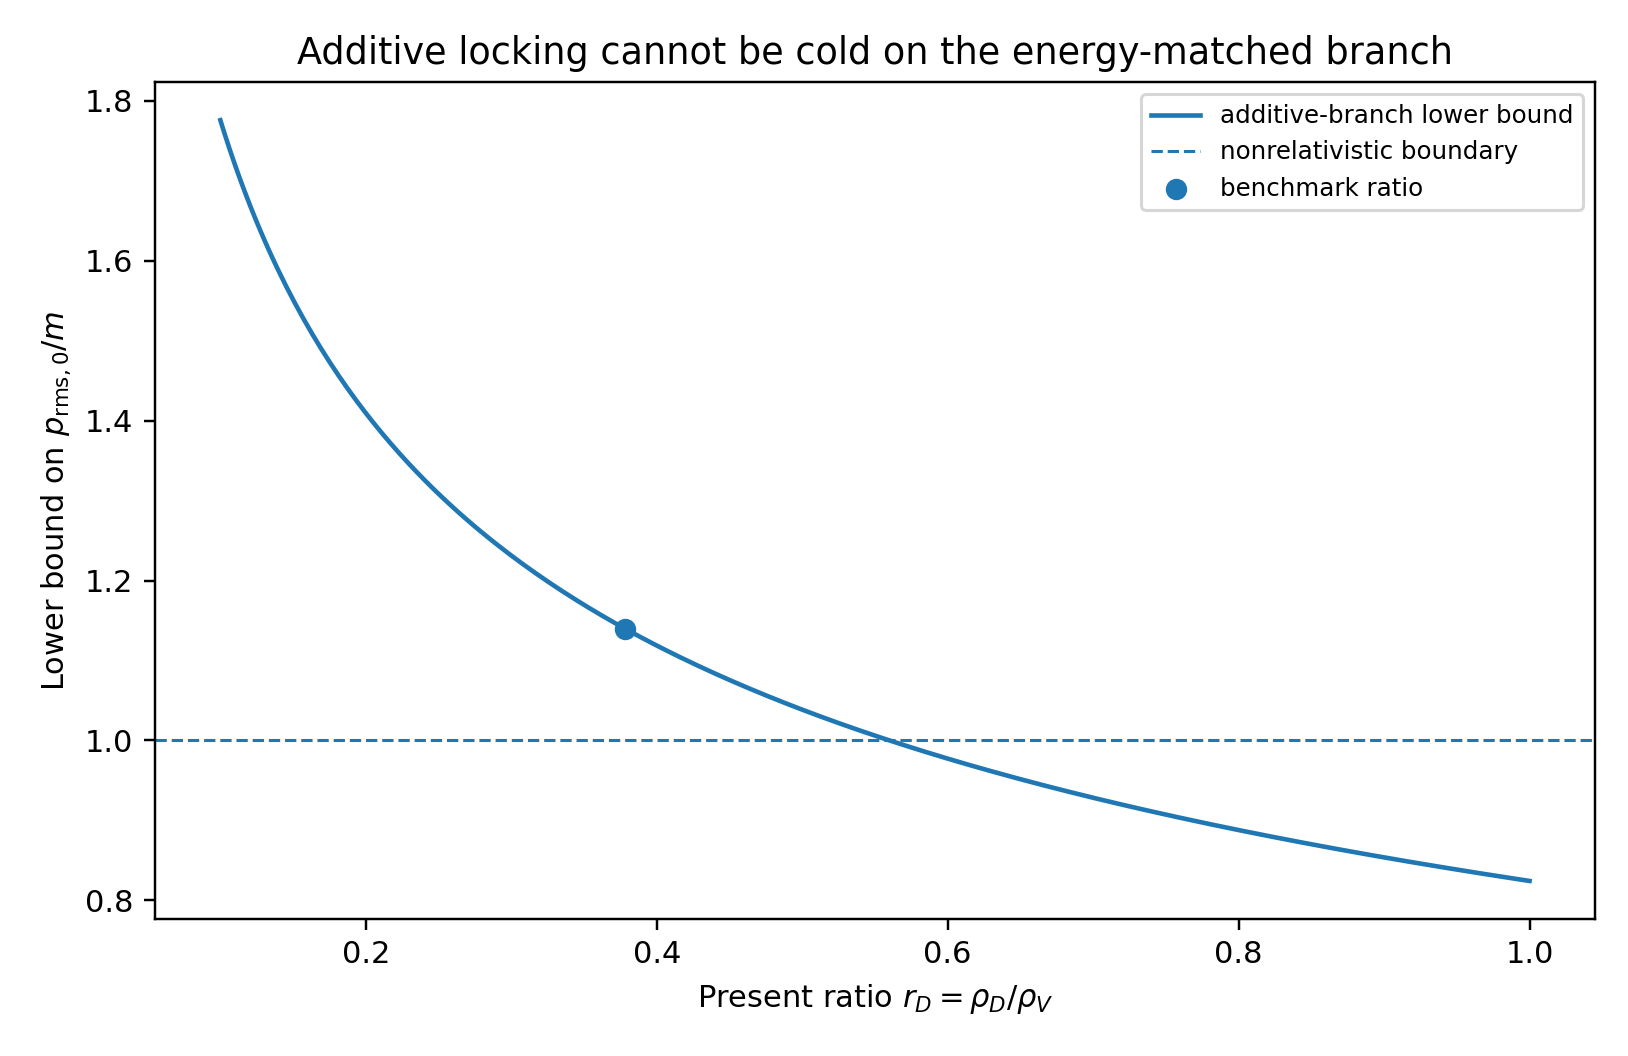
\includegraphics[width=0.90\linewidth]{figures/scw/additive_branch_obstruction.png}
\caption{The abundance, energy-matching, and locking conditions force the additive one-shell ratio $p_{\rm rms}/m$ above unity at the declared present density ratio, contradicting the assumed cold branch.}
\label{fig:scw-additive-obstruction}
\end{figure}

\section{Scale-covariant fiber action}

Let
\begin{equation}
 U(\phi)=\frac{\lambda}{4}(\phi^2-v^2)^2,
 \qquad
 \mu^2=\lambda v^2,
 \label{eq:scw-average-potential}
\end{equation}
and let
\begin{equation}
 \mathcal L_{\sigma,p}
 =\Lambda^2\sum_{h\geq1}p^{2\sigma h}\mathsf D_h.
 \label{eq:scw-fiber-operator}
\end{equation}
The scale-covariant branch is defined by
\begin{equation}
\boxed{
\begin{aligned}
 S_{\rm SC}
 =-\int\sqrt{-g}\,d^4x\Bigg[
 &\frac12(\partial\phi)^2+U(\phi)
 +\frac12\langle\partial\chi,\partial\chi\rangle_p\\
 &+\frac12\left\langle
 \chi,
 \left(
 m_0^2-\mu^2
 +\left(1+\gamma\frac{\phi^2}{v^2}\right)
 \mathcal L_{\sigma,p}
 \right)\chi
 \right\rangle_p
 \Bigg].
\end{aligned}}
 \label{eq:scw-action}
\end{equation}
The level masses at the locked origin are
\begin{equation}
 m_h^2
 =m_0^2-\mu^2+\Lambda^2p^{2\sigma h},
 \label{eq:scw-level-masses}
\end{equation}
with multiplicities
\begin{equation}
 d_h=(p-1)p^{h-1}.
 \label{eq:scw-level-degeneracy}
\end{equation}
The average mode now changes the internal refinement scale itself.  Its homogeneous equation is
\begin{equation}
 \ddot\phi+3H\dot\phi
 +\lambda\phi(\phi^2-v^2)
 +\frac{\gamma\phi}{v^2}Y_D=0,
 \label{eq:scw-average-eom}
\end{equation}
where
\begin{equation}
 Y_D
 :=\sum_h\Lambda^2p^{2\sigma h}X_h,
 \qquad
 X_h:=\langle\chi_h^2\rangle.
 \label{eq:scw-weighted-lock-source}
\end{equation}
The origin curvature is
\begin{equation}
 \boxed{
 M_\phi^2
 =-\mu^2+\frac{\gamma}{v^2}Y_D.}
 \label{eq:scw-lock-curvature}
\end{equation}
For nonrelativistic levels with $m_h^2\gg\mu^2,m_0^2$,
\begin{equation}
 \Lambda^2p^{2\sigma h}X_h
 =\rho_h\left[1+O(w_h)+O\left(\frac{\mu^2+m_0^2}{m_h^2}\right)\right].
 \label{eq:scw-weighted-energy-limit}
\end{equation}
Thus the total cold dark density, including heavy levels, supplies the locking source.

\section{Weighted nonadiabatic production}

Near a crossing,
\begin{equation}
 \phi(t)=\dot\phi_\star(t-t_\star)+O((t-t_\star)^2),
 \label{eq:scw-crossing-linearization}
\end{equation}
so that
\begin{equation}
 \omega_{h,k}^2
 =k^2+m_h^2
 +\frac{\gamma\Lambda^2p^{2\sigma h}}{v^2}
 \dot\phi_\star^2(t-t_\star)^2.
 \label{eq:scw-crossing-frequency}
\end{equation}
Define
\begin{equation}
 A_\star:=\frac{\sqrt\gamma|\dot\phi_\star|}{v},
 \qquad
 \nu_h:=A_\star\Lambda p^{\sigma h}.
 \label{eq:scw-weighted-rate}
\end{equation}
The rapid-crossing spectrum is
\begin{equation}
 \boxed{
 f_h(k)
 =\eta
 \exp\left[-\frac{\pi(k^2+m_h^2)}{\nu_h}\right],}
 \label{eq:scw-weighted-occupation}
\end{equation}
where $\eta$ is fixed by energy projection when the linearized spectrum would exceed the available kinetic energy:
\begin{equation}
 \eta
 =\min\left(1,\frac{K_\star}{\widetilde\rho_\star}\right).
 \label{eq:scw-energy-projection}
\end{equation}
This is not an independent abundance fit.  It is the shape-preserving rapid-crossing approximation with exact total-energy matching.

At high level,
\begin{equation}
 m_h\simeq\Lambda p^{\sigma h},
 \qquad
 \nu_h\simeq A_\star m_h.
 \label{eq:scw-high-level-law}
\end{equation}
The suppression exponent becomes linear rather than quadratic in mass:
\begin{equation}
 \frac{\pi m_h^2}{\nu_h}
 \simeq\frac{\pi m_h}{A_\star}.
 \label{eq:scw-linear-mass-suppression}
\end{equation}
At the same time,
\begin{equation}
 \frac{p_{\rm rms,\star}}{m_h}
 \simeq
 \sqrt{\frac{3A_\star}{2\pi m_h}},
 \label{eq:scw-heavy-colder}
\end{equation}
so heavier populated levels are born colder.

\section{Exact \texorpdfstring{$\sigma=1$}{sigma=1} continuum theorem}

For $\sigma=1$, the endpoint law
\begin{equation}
 N(m)=\frac{m}{\Lambda}-1
 \label{eq:scw-state-count}
\end{equation}
gives the continuum density of levels
\begin{equation}
 \frac{dN}{dm}=\frac1\Lambda.
 \label{eq:scw-density-of-levels}
\end{equation}
Using $\nu=Am$ and the occupation \eqref{eq:scw-weighted-occupation}, the number and captured rest-density spectra are
\begin{equation}
 \frac{dn}{dm}
 =\eta\frac{A^{3/2}}{8\pi^3\Lambda}
 m^{3/2}e^{-\pi m/A},
 \label{eq:scw-number-spectrum}
\end{equation}
\begin{equation}
 \boxed{
 \frac{d\rho_R}{dm}
 =\eta\frac{A^{3/2}}{8\pi^3\Lambda}
 m^{5/2}e^{-\pi m/A}.}
 \label{eq:scw-rest-spectrum}
\end{equation}
The selected mass band peaks at
\begin{equation}
 \boxed{
 m_{\rm peak}=\frac{5A}{2\pi}.}
 \label{eq:scw-mass-peak}
\end{equation}
The exact continuum integrals are
\begin{equation}
 n_\star=C_N\eta\frac{A^4}{\Lambda},
 \qquad
 C_N=\frac{3}{32\pi^5},
 \label{eq:scw-number-constant}
\end{equation}
\begin{equation}
 \rho_{R,\star}=C_R\eta\frac{A^5}{\Lambda},
 \qquad
 C_R=\frac{15}{64\pi^6},
 \label{eq:scw-rest-constant}
\end{equation}
\begin{equation}
 \rho_\star=C_E\eta\frac{A^5}{\Lambda},
 \qquad
 C_E=\frac{32}{35\pi^7},
 \label{eq:scw-energy-constant}
\end{equation}
\begin{equation}
 p_\star=C_P\eta\frac{A^5}{\Lambda},
 \qquad
 C_P=\frac{32}{315\pi^7}.
 \label{eq:scw-pressure-constant}
\end{equation}
For example, the total-energy coefficient follows from the Tricomi representation and the beta integral:
\begin{equation}
\begin{aligned}
 C_E
 &=\frac{1}{2\pi^2}
 \int_0^\infty y^2e^{-\pi y}I_\rho(\sqrt y)\,dy\\
 &=\frac{6}{\pi^7}B\left(\frac32,3\right)
 =\frac{32}{35\pi^7}.
\end{aligned}
 \label{eq:scw-energy-beta-proof}
\end{equation}
Consequently,
\begin{equation}
 \boxed{
 w_\star=\frac{p_\star}{\rho_\star}=\frac19,}
 \label{eq:scw-production-w}
\end{equation}
\begin{equation}
 \boxed{
 f_R:=\frac{\rho_{R,\star}}{\rho_\star}
 =\frac{525\pi}{2048}
 =0.8053399136\ldots,}
 \label{eq:scw-rest-fraction}
\end{equation}
and
\begin{equation}
 \frac{\rho_{R,\star}}{n_\star}
 =\frac{5A}{2\pi}
 =m_{\rm peak}.
 \label{eq:scw-mean-mass}
\end{equation}

A dyadic discrete tower with $\Lambda/A=10^{-4}$ gives
\begin{equation}
 f_R^{(2)}=0.8054331018,
 \qquad
 w_\star^{(2)}=0.1110616168,
 \label{eq:scw-discrete-ratios}
\end{equation}
and selects
\begin{equation}
 \frac{m_{\rm peak}^{(2)}}A=0.8192,
 \label{eq:scw-discrete-peak}
\end{equation}
within one dyadic bin of \eqref{eq:scw-mass-peak}.  The absolute normalization retains the known log-periodic prime modulation, while the ratios are nearly envelope independent.

\begin{figure}[htbp]
\centering
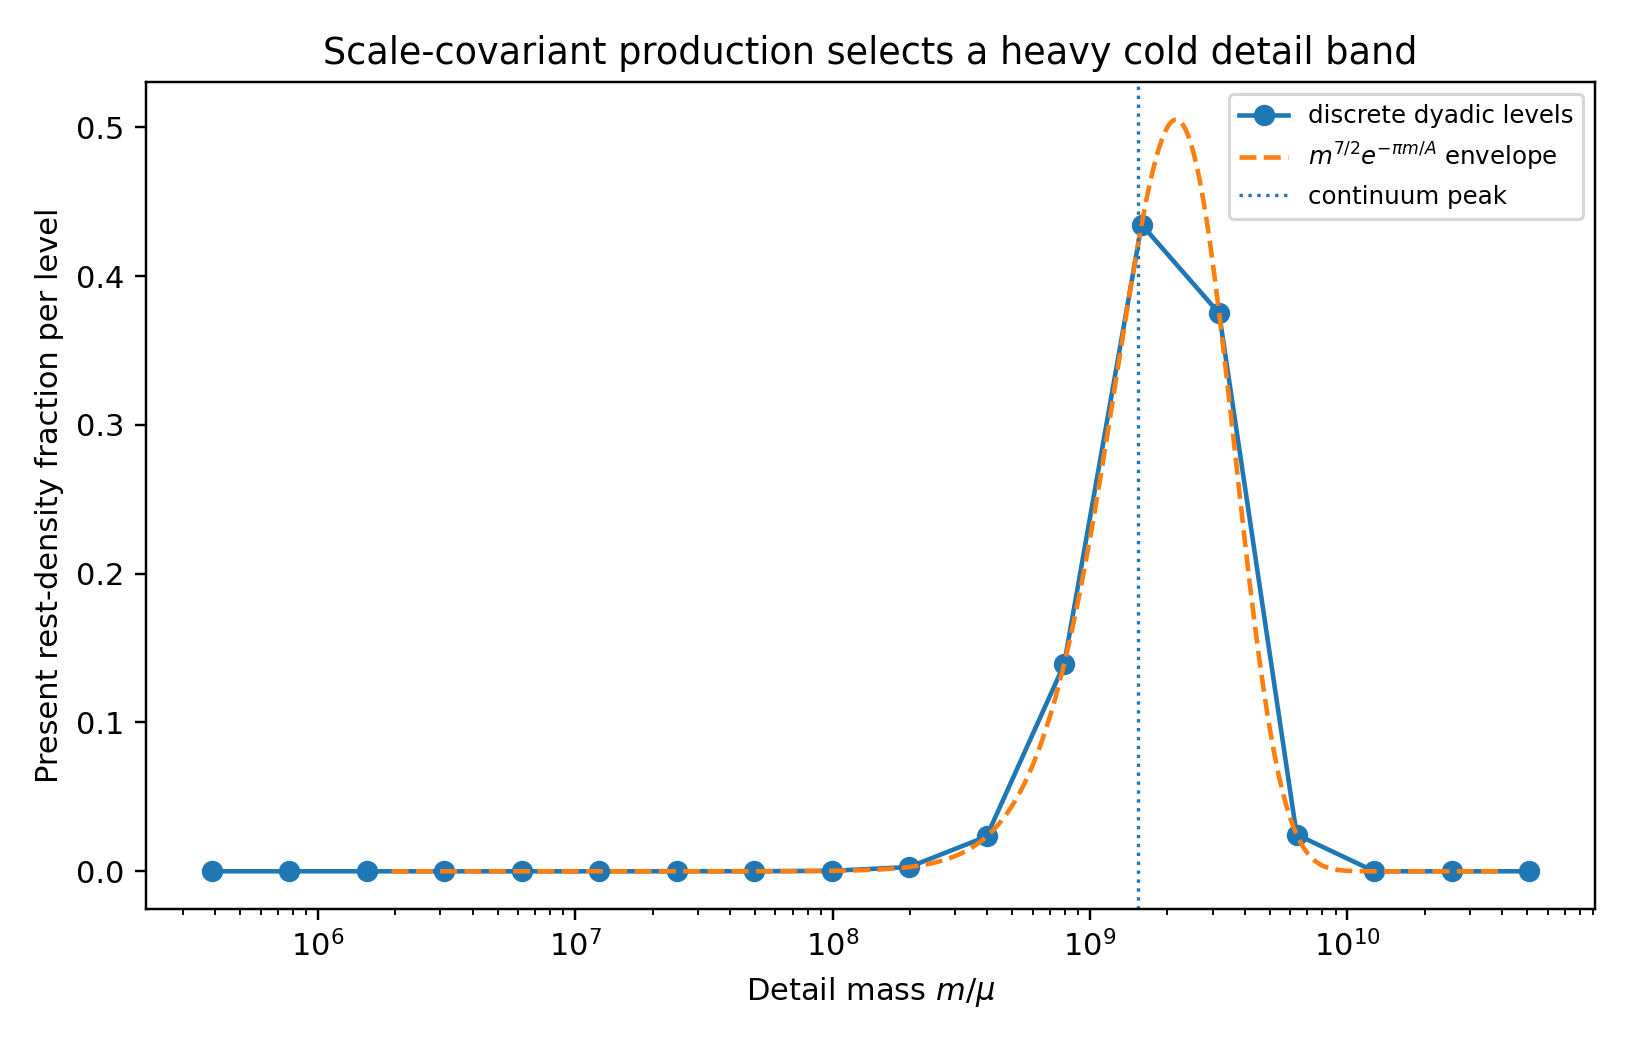
\includegraphics[width=0.92\linewidth]{figures/scw/weighted_detail_mass_spectrum.png}
\caption{The discrete dyadic rest-density fractions follow the analytic scale-covariant mass envelope.  The dominant mass is many orders of magnitude above the vacuum scale in the calibrated benchmark.}
\label{fig:scw-mass-spectrum}
\end{figure}

\section{Abundance calibration and emergent hierarchy}

On the captured branch,
\begin{equation}
 \rho_{R,\star}=f_RK_\star.
 \label{eq:scw-captured-rest}
\end{equation}
After the produced band becomes nonrelativistic,
\begin{equation}
 \rho_{D0}=f_RK_\star a_\star^3.
 \label{eq:scw-present-abundance}
\end{equation}
Define
\begin{equation}
 F:=\frac{K_\star}{\rho_V}.
 \label{eq:scw-F-definition}
\end{equation}
The present abundance fixes
\begin{equation}
 \boxed{
 F=\frac{r_D}{f_Ra_\star^3}.}
 \label{eq:scw-F-calibration}
\end{equation}
The crossing scale and selected mass are then
\begin{equation}
 \frac{A_\star}{\mu}
 =\sqrt{\frac{\gamma F}{2}},
 \label{eq:scw-A-over-mu}
\end{equation}
\begin{equation}
 \boxed{
 \frac{m_{\rm peak}}\mu
 =\frac{5}{2\pi}
 \sqrt{\frac{\gamma r_D}{2f_Ra_\star^3}}.}
 \label{eq:scw-peak-hierarchy}
\end{equation}
If the average field begins at rest at $\phi_i$, then
\begin{equation}
 F
 =\left(\frac{\phi_i}{v}\right)^4
 -2\left(\frac{\phi_i}{v}\right)^2,
 \label{eq:scw-initial-energy}
\end{equation}
so
\begin{equation}
 \boxed{
 \frac{|\phi_i|}{v}
 =\sqrt{1+\sqrt{1+F}}.}
 \label{eq:scw-initial-amplitude}
\end{equation}
Thus one early production scale determines both the hierarchy between the vacuum and dark-matter masses and the required pre-crossing field amplitude.

For the benchmark
\begin{equation}
 a_\star=10^{-6},
 \qquad
 \gamma=16,
 \qquad
 p=2,
 \qquad
 \frac{\Lambda}{A_\star}=10^{-4},
 \label{eq:scw-benchmark-inputs}
\end{equation}
with \eqref{eq:scw-rd-benchmark}, the discrete calculation gives
\begin{equation}
 \frac{K_\star}{\rho_V}
 =4.6969787254\times10^{17},
 \label{eq:scw-benchmark-F}
\end{equation}
\begin{equation}
 \frac{A_\star}{\mu}
 =1.9384486014\times10^9,
 \qquad
 \frac{|\phi_i|}{v}=2.6179096175\times10^4,
 \label{eq:scw-benchmark-hierarchy}
\end{equation}
\begin{equation}
 \boxed{
 \frac{m_{\rm peak}^{(2)}}\mu
 =1.5879770943\times10^9.}
 \label{eq:scw-benchmark-peak}
\end{equation}
The shape-preserving energy projection is
\begin{equation}
 \eta=3.8062069178\times10^{-21}.
 \label{eq:scw-benchmark-eta}
\end{equation}
This small occupation per microscopic state is compensated by the large refinement multiplicities.  It is determined by energy conservation after the rapid-crossing spectrum is assembled.

\section{Coldness theorem and cutoff scale}

At $a\gg a_\star$, the scale-covariant continuum band obeys
\begin{equation}
 \boxed{
 w_D(a)=\frac{a_\star^2}{5a^2},}
 \label{eq:scw-late-w}
\end{equation}
\begin{equation}
 \boxed{
 c_{a,D}^2(a)=\frac{a_\star^2}{3a^2},}
 \label{eq:scw-late-ca}
\end{equation}
and
\begin{equation}
 \boxed{
 v_{\rm rms}(a)
 =\sqrt{\frac35}\frac{a_\star}{a}.}
 \label{eq:scw-late-speed}
\end{equation}
Unlike the additive one-shell result, the present speed decreases directly with the production scale.  The reason is that the selected mass grows with the crossing rate while its fractional production momentum decreases as $m^{-1/2}$.

For $a_\star=10^{-6}$,
\begin{equation}
 w_{D0}=1.9987378335\times10^{-13},
 \qquad
 v_{\rm rms,0}=7.7459666924\times10^{-7}.
 \label{eq:scw-benchmark-coldness}
\end{equation}
The fluid Jeans estimate is
\begin{equation}
 \frac{k_J(a)}{aH(a)}
 =\sqrt{\frac{3\Omega_m(a)}{2c_{a,D}^2(a)}},
 \label{eq:scw-jeans-definition}
\end{equation}
which gives
\begin{equation}
 \boxed{
 \frac{k_J(a)}{H_0}
 =\frac{3}{\sqrt2}
 \frac{\sqrt{\Omega_{m0}a}}{a_\star}.}
 \label{eq:scw-jeans-law}
\end{equation}
At the present epoch,
\begin{equation}
 \frac{k_{J0}}{H_0}=1.1811011811\times10^6.
 \label{eq:scw-benchmark-jeans}
\end{equation}

\section{Density locking and transient acceleration}

Using \eqref{eq:scw-weighted-energy-limit}, the locked cold branch satisfies
\begin{equation}
 \frac{M_\phi^2}{\mu^2}
 =-1+\frac{\gamma}{4}r_D(a)
 +O(w_D)+O\left(\frac{\mu^2}{m_{\rm eff}^2}\right).
 \label{eq:scw-lock-density-law}
\end{equation}
Hence present locking requires
\begin{equation}
 \boxed{
 \gamma>\frac{4}{r_{D0}}.}
 \label{eq:scw-gamma-lock}
\end{equation}
For the declared ratio, the right side is $10.573\ldots$.  The benchmark choice $\gamma=16$ gives
\begin{equation}
 \boxed{
 \frac{M_\phi^2(1)}{\mu^2}=0.5132408576.}
 \label{eq:scw-present-lock-curvature}
\end{equation}
The exact discrete kinetic moments reconstruct
\begin{equation}
 \frac{Y_D(1)}{\rho_V}=0.3783102144
 \label{eq:scw-weighted-source-numeric}
\end{equation}
within $2.3\times10^{-13}$ of the declared dark-density ratio.

The cold asymptotic release scale is
\begin{equation}
 a_{\rm release}
 =\left(\frac{\gamma r_{D0}}4\right)^{1/3}.
 \label{eq:scw-release-law}
\end{equation}
The exact discrete result is
\begin{equation}
 \boxed{
 a_{\rm release}=1.1480726020.}
 \label{eq:scw-release-numeric}
\end{equation}
For baryon ratio
\begin{equation}
 r_{b0}=0.0710237567,
 \label{eq:scw-rb-benchmark}
\end{equation}
the acceleration onset is
\begin{equation}
 \boxed{
 a_{\rm acc}=0.6081134084,}
 \label{eq:scw-acceleration-numeric}
\end{equation}
with a cold asymptotic estimate differing by $1.94\times10^{-4}$.

At the locked point, the quadratic average-mode action remains
\begin{equation}
 S_{\delta\phi}^{(2)}
 =\frac12\int a^3dt\,d^3x
 \left[
 \delta\dot\phi^2
 -\frac{(\nabla\delta\phi)^2}{a^2}
 -M_\phi^2\delta\phi^2
 \right].
 \label{eq:scw-perturbation-action}
\end{equation}
Therefore
\begin{equation}
 Q_{\delta\phi}=1,
 \qquad
 c_{s,\phi}^2=1,
 \qquad
 M_\phi^2>0
 \label{eq:scw-perturbation-stability}
\end{equation}
throughout the locked interval.  Because every mass deformation is even in $\phi$, the detail stress tensor also has no term linear in $\delta\phi$ at $\phi=0$.

\begin{figure}[htbp]
\centering
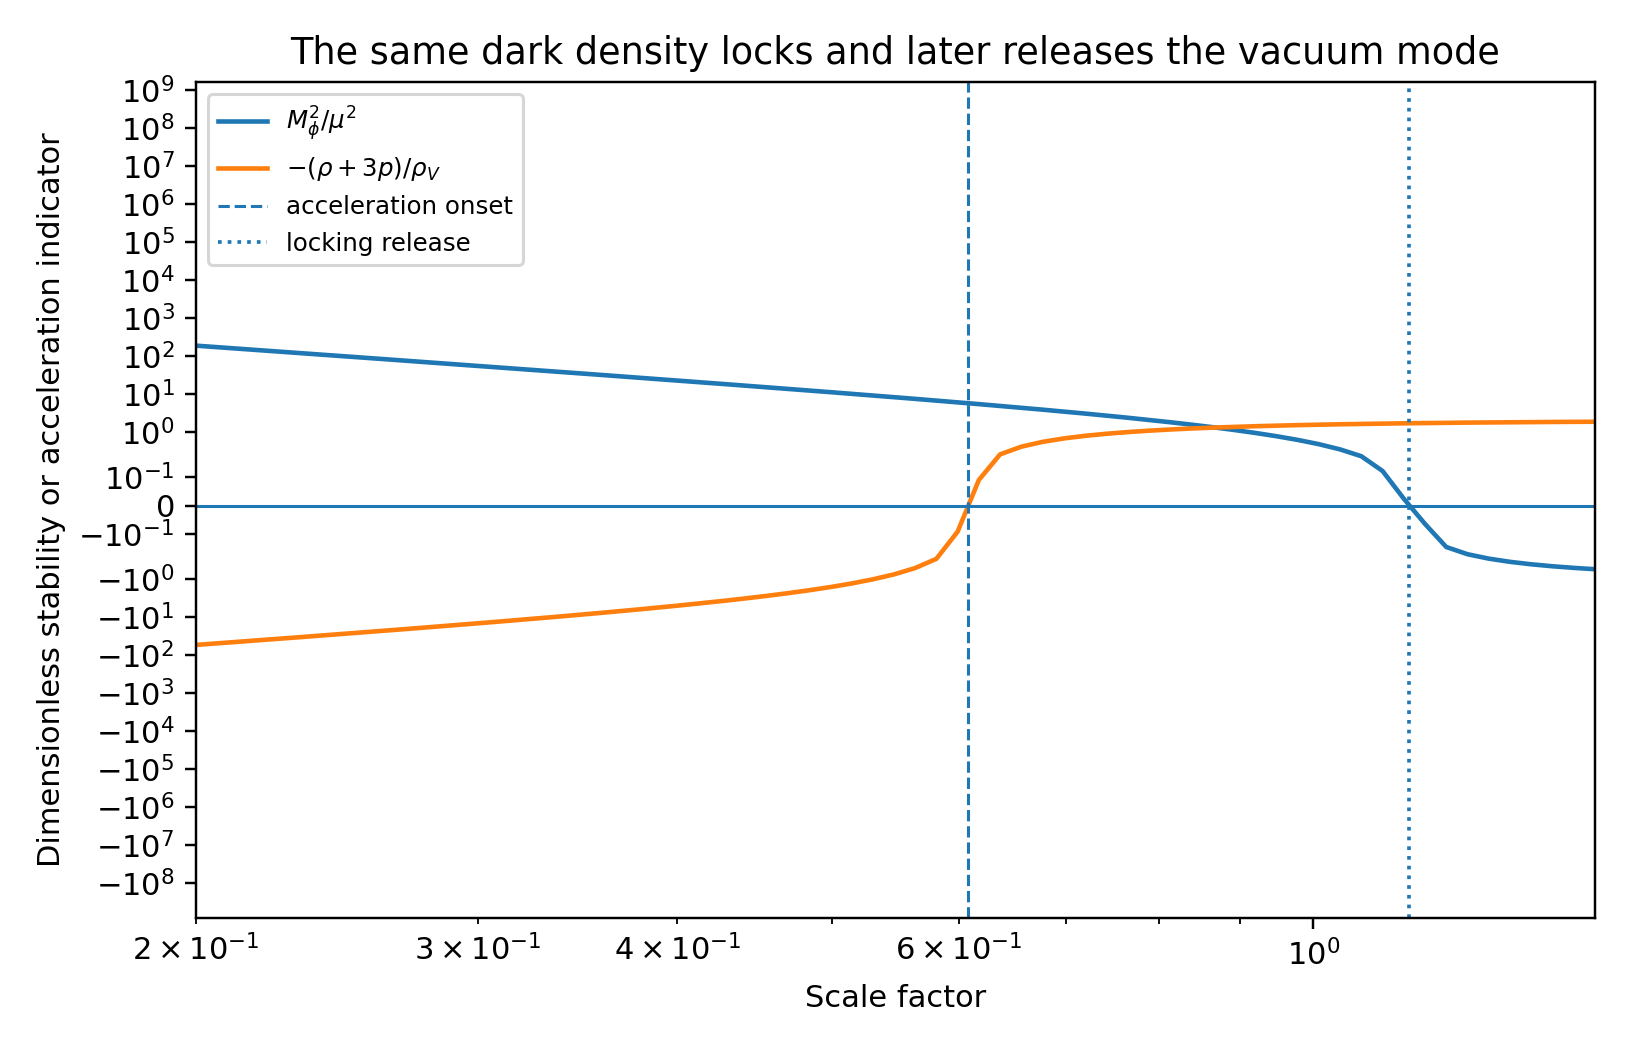
\includegraphics[width=0.92\linewidth]{figures/scw/weighted_locking_and_release.png}
\caption{The weighted detail density stabilizes the average mode well before acceleration begins.  Dilution eventually removes the locking curvature and releases the vacuum mode.}
\label{fig:scw-lock-release}
\end{figure}

\section{Linear growth and lensing benchmark}

For $a\gg a_\star$, use $N=\log a$ and the controlled cold-fluid closure
\begin{equation}
 \delta_b''
 +\left(2+\frac{d\log H}{dN}\right)\delta_b'
 =\frac32S,
 \label{eq:scw-baryon-growth}
\end{equation}
\begin{equation}
 \delta_D''
 +\left(2+\frac{d\log H}{dN}\right)\delta_D'
 +\frac{c_{a,D}^2k^2}{a^2H^2}\delta_D
 =\frac32S,
 \label{eq:scw-dark-growth}
\end{equation}
where
\begin{equation}
 S=\Omega_b(a)\delta_b+\Omega_D(a)\delta_D.
 \label{eq:scw-growth-source}
\end{equation}
The same source controls the subhorizon lensing potential to the accuracy of this closure.

Starting at $a_i=10^{-3}$ with adiabatic growing data, the benchmark gives
\begin{center}
\begin{tabular}{rcc}
\toprule
$k/H_0$ & $\delta_D/\delta_{D,{\rm cold}}$ & lensing source / cold source\\
\midrule
$30$ & $0.9999996989$ & $0.9999997007$\\
$300$ & $0.9999698901$ & $0.9999700727$\\
$3000$ & $0.9969926202$ & $0.9970108463$\\
$10000$ & $0.9669918115$ & $0.9671896257$\\
$30000$ & $0.7331608409$ & $0.7346038042$\\
$100000$ & $0.0159173474$ & $0.0169297429$\\
\bottomrule
\end{tabular}
\end{center}
The first half-mode of the fluid lensing-source transfer is
\begin{equation}
 \boxed{
 \frac{k_{1/2}}{H_0}=4.4076353413\times10^4.}
 \label{eq:scw-half-mode}
\end{equation}
For the conditional conversion $H_0=70\,\mathrm{km\,s^{-1}\,Mpc^{-1}}$,
\begin{equation}
 k_{1/2}=10.2916022620\,\mathrm{Mpc}^{-1}.
 \label{eq:scw-half-mode-mpc}
\end{equation}
This is a fluid-closure benchmark, not yet a complete collisionless Einstein--Boltzmann likelihood.

\begin{figure}[htbp]
\centering
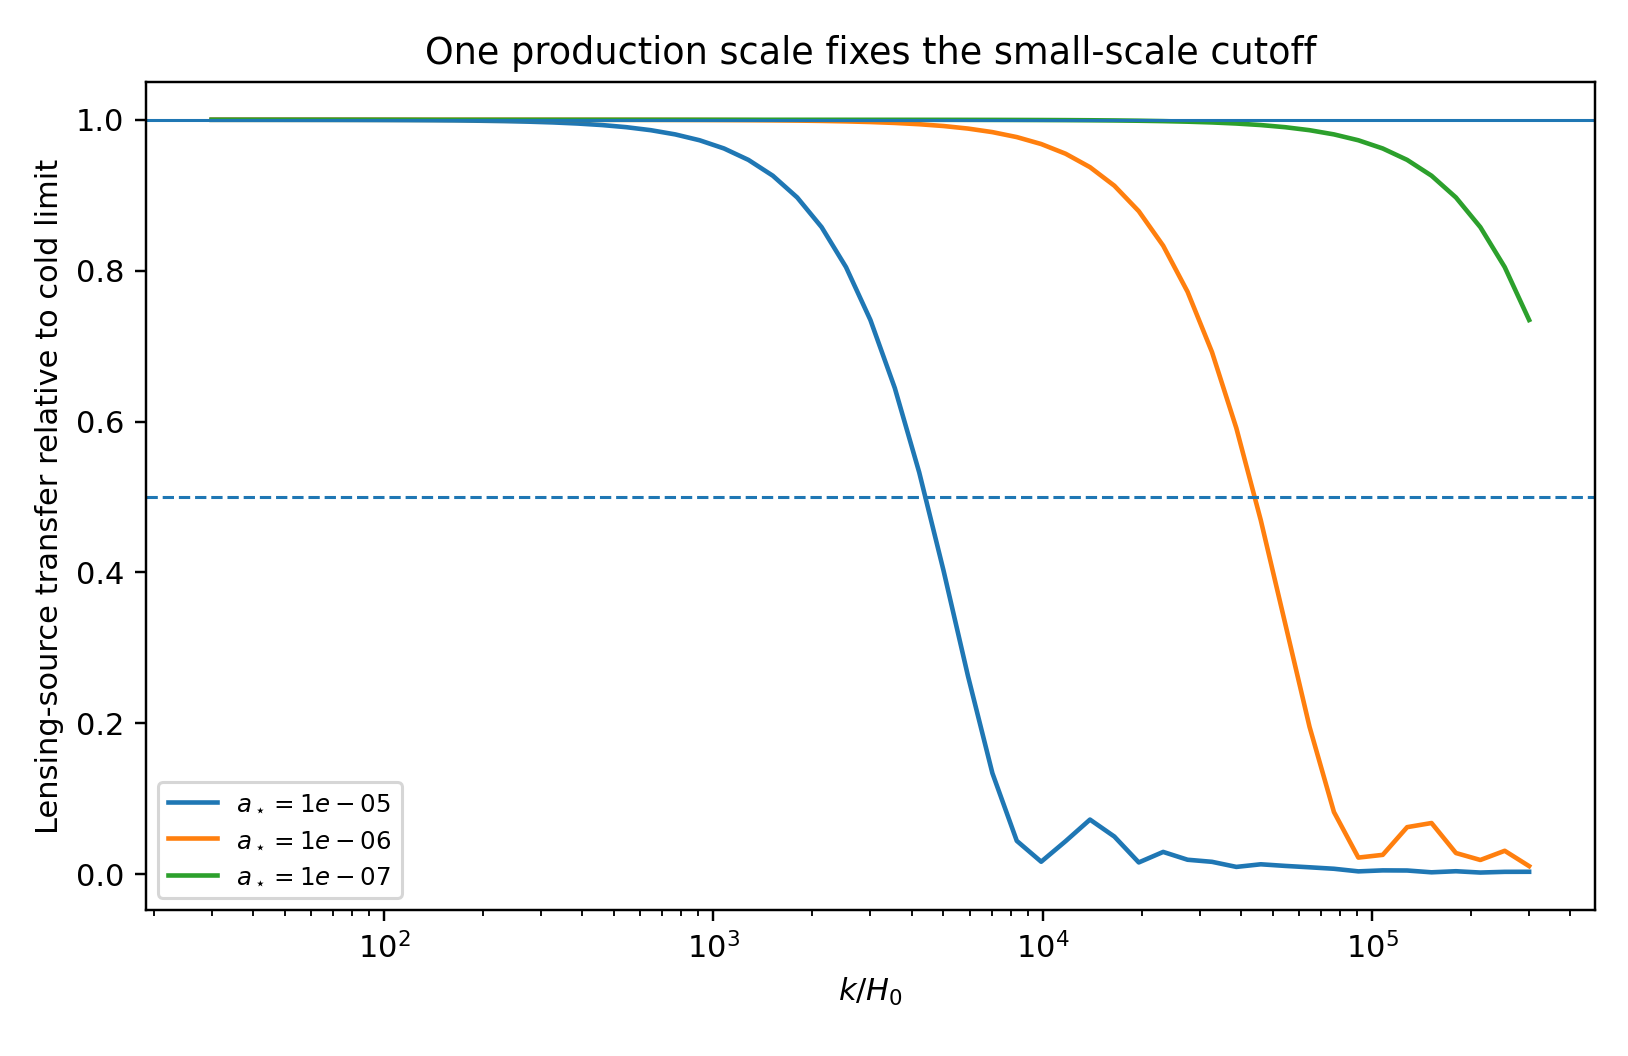
\includegraphics[width=0.92\linewidth]{figures/scw/weighted_transfer_suppression.png}
\caption{The production epoch controls the free-streaming cutoff without changing the late locking law.  The high-$k$ oscillations are those of the finite sound-speed fluid closure.}
\label{fig:scw-transfer}
\end{figure}

\section{Verification ledger}

The deterministic calculation records twenty passes and no failures.  Selected checks are
\begin{center}
\begin{tabular}{p{0.64\linewidth}r}
\toprule
statement & residual\\
\midrule
additive abundance--velocity elimination identity & $0$\\
continuum $C_E$ versus independent quadrature & $1.62\times10^{-12}$ relative\\
continuum $C_P$ versus independent quadrature & $3.49\times10^{-11}$ relative\\
discrete versus continuum captured rest fraction & $9.32\times10^{-5}$\\
discrete versus continuum production $w$ & $4.95\times10^{-5}$\\
present abundance reconstruction & $0$\\
exact versus asymptotic release scale & $1.95\times10^{-13}$\\
exact versus asymptotic acceleration scale & $1.93\times10^{-4}$\\
exact kinetic $c_a^2$ versus $a_\star^2/(3a^2)$ & $6.31\times10^{-4}$ relative\\
large-scale lensing-source deviation at $k/H_0=300$ & $2.99\times10^{-5}$\\
\bottomrule
\end{tabular}
\end{center}
The executable records are
\begin{equation}
 R_{\rm SC}=\texttt{data/Scale\_Covariant\_Dark\_Sector\_Verification.json},
 \label{eq:scw-json-record}
\end{equation}
\begin{equation}
 C_{\rm SC}=\texttt{data/scale\_covariant\_dark\_checks.csv},
 \label{eq:scw-check-record}
\end{equation}
\begin{equation}
 X_{\rm SC}=\texttt{verification/Scale\_Covariant\_Dark\_Sector\_Verification.py}.
 \label{eq:scw-script-record}
\end{equation}

\section{Closure ledger and remaining burden}

\begin{center}
\begin{tabular}{@{}>{\raggedright\arraybackslash}p{0.47\linewidth}>{\raggedright\arraybackslash}p{0.18\linewidth}>{\raggedright\arraybackslash}p{0.27\linewidth}@{}}
\toprule
statement & status & boundary\\
\midrule
additive one-shell cold-lock obstruction & proved conditional & rapid, energy-matched, dominant-shell branch\\
scale-covariant fiber action & defined & one new coupling $\gamma$\\
weighted production spectrum & derived & linear rapid crossing\\
$\sigma=1$ continuum mass theorem & proved & high-level density-of-states envelope\\
energy-projected rest fraction & proved & shape-preserving capture approximation\\
late $w_D$, $c_a^2$, and $v_{\rm rms}$ laws & proved asymptotically & collisionless nonrelativistic regime\\
density locking and release & closed controlled & heavy-level limit and regular locked phase\\
linear growth and lensing cutoff & numerical controlled & two-fluid sound-speed closure\\
full collisionless hierarchy & open & momentum and anisotropic-stress multipoles\\
radiative stability of scale covariance & open & quantum effective action\\
microscopic derivation of $\gamma$ and $a_\star$ & open & gravitational refinement dynamics\\
observational likelihood and priority audit & open & independent implementation and data comparison\\
\bottomrule
\end{tabular}
\end{center}

The principal result is not that every earlier dark-sector formula survives unchanged.  The hard consistency audit rejects the additive dominant-shell mechanism and identifies a minimal viable replacement:
\begin{equation}
 \boxed{
 \begin{gathered}
 \text{average-mode dilation of the refinement spectrum}\\
 \Longrightarrow \text{ heavy cold detail band}\\
 \Longrightarrow \text{ density-weighted vacuum locking}
 \end{gathered}}
 \label{eq:scw-result-chain}
\end{equation}
A complete physical treatment therefore requires the full collisionless Einstein--Boltzmann hierarchy for the distribution \eqref{eq:scw-weighted-occupation}, with one parameter set propagated through recombination, matter power, weak lensing, and the transient-release background without sector-by-sector renormalization.
